\section{Introduction}
The Measurement Network Gateway (MNG) is one of the embedded measurement platform designed which to collect different types of sensor data, process it in real time, and transmit the resulting measurements over an Ethernet network to a remote client. The system is designed for applications that need consistent sampling, accurate timing, and easy integration with a Linux-based software environment. To satisfy these requirements, the MNG hardware architecture combines a System-on-Chip (SoC) processing platform with dedicated measurement peripherals and standardized communication interfaces. The hardware uses a layered architecture: time-critical and low-level signal operations run close to the hardware, while higher-level control, data processing, and networking are handled in software. Analog voltages are measured with the PmodAD1 ADC module,  for temperature measurement we are using a MAX31865 RTD interface, and digital inputs are read from switches and buttons. Precise and adjustable sampling rates are generated using clocked logic and on-chip timers, ensuring predictable behavior independent of the operating system.

To provide a clean and safe interface between hardware and software, all measurement and control functions are abstracted as memory-mapped registers behind a custom measurement interface IP core. Low-level hardware functions which are SPI communication, ADC timing, GPIO control, and synchronization inside the FPGA handled, when Linux interacts with the system through a dedicated character device interface (/dev/meascdd). This way of approaching will hide the low level complexity form the user space software, also improves the system robustness, and able as for the future improvement  and extension without changing the fundamental architecture.

The below section will describe and explain the complete hardware architecture of Measurement Network Gateway, including the processing platform, sensor interfaces, timing and synchronization mechanisms, digital I/O, network connectivity, and validation methodology.

\section{Overall Hardware Architecture}
\subsection{Overview}
The hardware architecture of the Measurement Network Gateway is based and centered on a Zynq-7000 System-on-Chip that integrates a dual-core ARM processing system (PS) and FPGA-based programmable logic (PL) on a single device. This tightly integrated architecture enables time-critical measurement tasks to run in hardware, while high-level control and communication are handled by software under embedded Linux. External sensor modules and user interface components are connected to the Zynq platform using standardized interfaces such as SPI and GPIO.

In this system, every measurement follows a well-defined and consistent data path. A physical signal, such as an analog voltage, temperature-dependent resistance, or digital switch state, is first converted into a digital representation by the appropriate front-end device. Analog voltages are sampled by the PmodAD1 ADC, while temperature measurements are obtained through the MAX31865 RTD-to-digital converter. These digital data streams are then handled by custom logic inside the FPGA, where SPI communication timing, conversion control, and data latching are implemented deterministically.

The FPGA stores each completed measurement in memory-mapped registers that are connected to the AXI bus. These registers form the interface between the hardware and the processing system. On the PS side, a Linux device driver exposes this register interface through the /dev/meascdd device file, translating simple read and write operations on structured data into AXI register accesses. User-space software reads the measurements, places them into ring buffers, and forwards them over a TCP/IP connection to a graphical client.

All time-critical operations are confined to the hardware domain up to and including the FPGA registers. This includes ADC sampling, SPI state machines, conversion completion signaling, and enforcement of sensor-specific sampling frequencies. Higher-level tasks like drivers, buffering, networking, and visualization are not time-critical and can tolerate millisecond jitter, allowing precise measurements without sacrificing Linux flexibility.

\begin{figure}[H]
\centering 
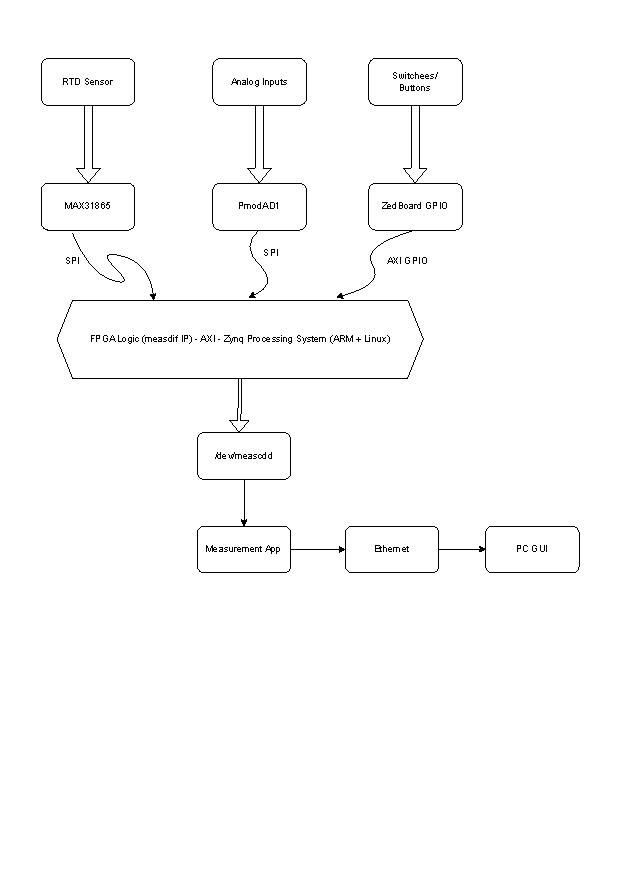
\includegraphics[width = 0.8\textwidth, trim = 0cm 4.5cm 0cm 0cm, clip]{media/hardArch.pdf}
\caption{Overall Hardware Architecrue of the Measurement Network Gateway}
\label{fig-reza1}
\end{figure}

\section{Zynq-7000 System-On-Chip Platform}
For the Measurement Network Gateway project the hardware implementation is based on only ZedBoard development platform that incorporates a Xilinx Zynq-7000 SoC. There are comprehensive set of  peripherals, including DDR3 memory, Ethernet connectivity, user input/output devices, and PMOD expansion connectors in this board. These features make the ZedBoard well suited for rapid prototyping of embedded measurement systems.

The ZedBoard acts as the central control unit of the system, hosting both the hardware interfaces implemented in programmable logic and the software environment running on the processing system. All external sensors and peripherals are physically connected to the ZedBoard, making it the focal point of the hardware design.

\begin{table}[H]
\centering 
\begin{tabularx}{\textwidth}{|X|X|X|}
\hline 
\textbf{Component} & \textbf{Purpose} & \textbf{Details} \\ \hline 
Dual ARM Cortex-A9 & Main Processor & Runs Linux kernel and application software \\ \hline 
FPGA Fabric & Custom Logic & Implements sensor interfaces, registers, timing logic \\ \hline  
DDR3 Memory & RAM & System memory for kernel and applications \\ \hline 
Ethernet MAC & Network Interface & Connects to lab network for TCP/IP communications \\ \hline 
GPIO Pins & Input / Output & User LEDs, switches, push buttons \\ \hline 
PMOD Headers & Expansions & Connectors for daughter boards (PmodAD1, MAX31865) \\ \hline 
\end{tabularx}
\caption{The Key Components on ZedBoard}
\end{table}

\begin{figure}[H]
\centering
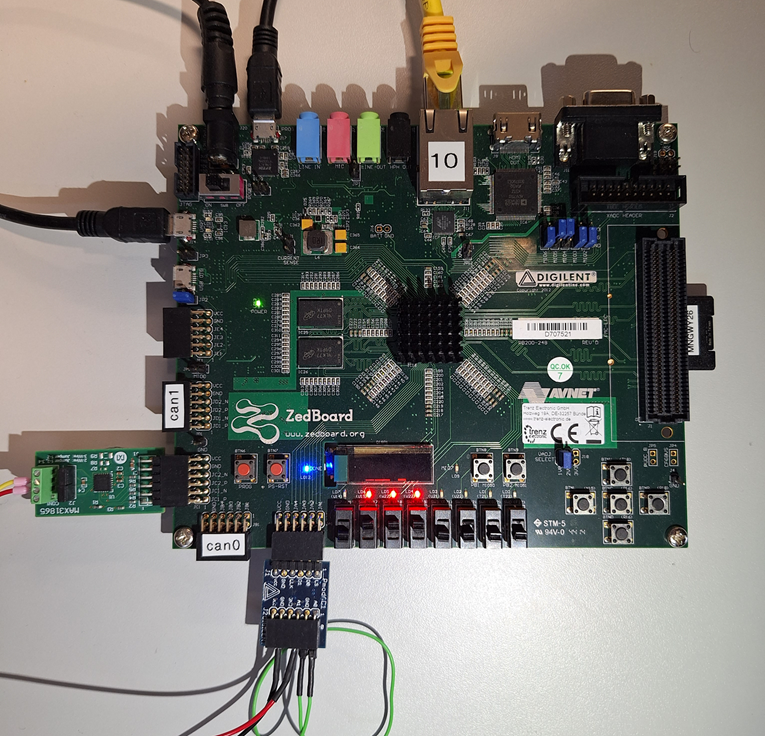
\includegraphics[width = \textwidth]{media/boardWithPeriph.png}
\caption{Zedboard development platform with connected peripherals}
\end{figure}

\subsection{Processing System}
In the processing system of Zynq-700, there is ARM Cortex-A9 processor running a Linux operating system generated using PetaLinux. This part of the system is responsible for the measurement application, managing network communication, and providing controlled access to hardware resources.

Linux is providing the stable runtime environment with a mature TCP/IP networking stack and a standardized device model. Hardware peripherals implemented in the programmable logic are exposed to user space through the /dev/meascdd character device and it allows the measurement application to contact with sensor for the read and write operations. With this approach, it is going to simplifies application development, improves portability, and separates hardware complexity from application logic.

So finally the process system is suited for those tasks that involves with complex protocols or variable execution timing which are such as TCP communication, command parsing, buffering, and interaction with a graphical user interface.

\subsection{Programming Logic (PL)}
In this part which is the programmable logic portion of the Zynq-7000 SoC, responsible for custom hardware interfaces for sensor communication and digital input/output. These interfaces are connected to the processing system via AXI interconnects, and they are enabling memory-mapped access to hardware registers.

For the measurement network gateway project the programmable logic implements SPI controllers for the PmodAD1 analog-to-digital converter and the MAX31865 RTD interface, as well as GPIO registers for switches, pushbuttons, and LEDs. The hardware is handling the Timing generation, conversion control, and status signaling. With the implementation of those functions in the FPGA fabric, the system achieves deterministic timing behavior and minimizes CPU load.

Programmable logic runs on its own clocks, independent of Linux, for precise sampling, parallel I/O, and dependable hardware interaction.
\begin{figure}[H]
	\centering 
	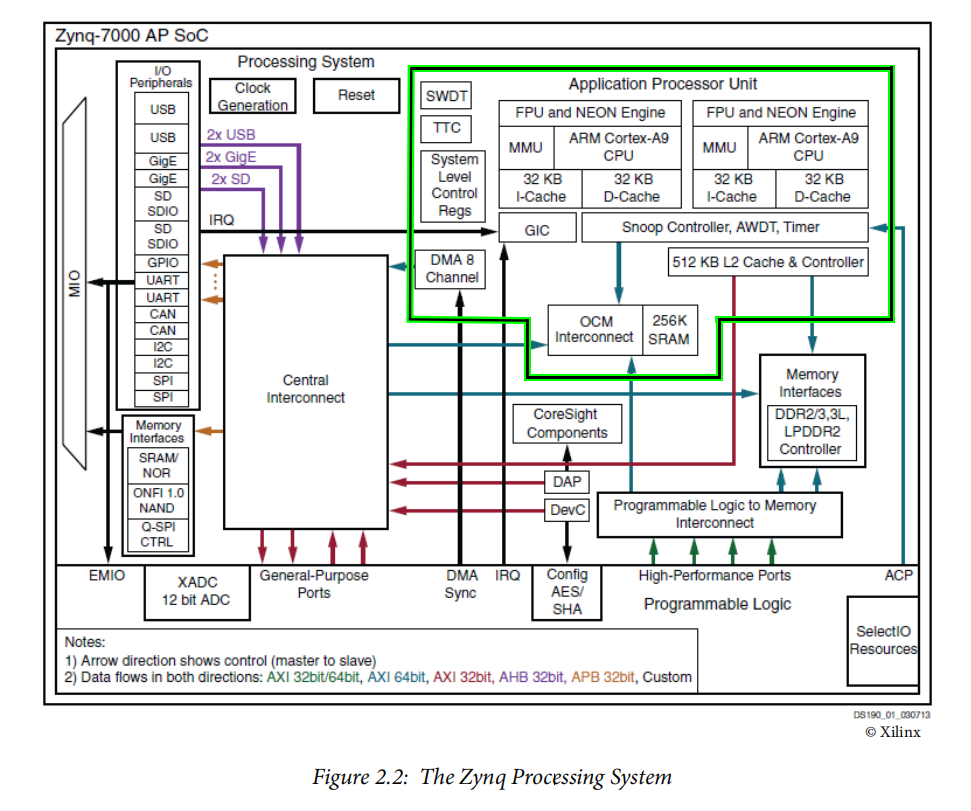
\includegraphics[width = 0.8\textwidth, trim = 0cm 1.5cm 0cm 0cm, clip]{media/processing.png}
	\caption{Zynq-7000 processing system architecture}
	\label{fig-zynq7000}
\end{figure}
	
\subsection{Division of Responsibilities between PS and PL}
The Zynq architecture distributes system functions between the Processing System (PS) and Programmable Logic (PL) based on timing requirements, implementation complexity, and suitability to hardware or software execution.

Time-Critical Functions in PL:
ADC signal acquisition and SPI communication are implemented in programmable logic because they require deterministic microsecond-scale timing. SPI bit clocks, chip-select windows, conversion start pulses, and sampling cadences must follow exact hardware timing constraints that are difficult to guarantee in software running under a preemptive operating system such as Linux. The FPGA fabric operates synchronously in well-defined clock domains, allowing sensor interfaces and GPIO sampling to execute independently of CPU load and operating system scheduling.

\subsubsection{High-Level Functions in PS}
In contrast, network communication and application logic are implemented in the processing system. TCP/IP protocol handling, socket management, command parsing, and ring buffer management involve complex, stateful operations that benefit from the mature Linux networking stack and device driver model. These functions tolerate millisecond-scale jitter without affecting measurement quality, making them well suited for execution in software on the ARM processor.

\subsubsection{Register Interface as the Bridge}
Memory-mapped registers serve as the clean boundary between hardware and software. PL logic based on its own clock domain is updating continuously sensor measurement registers, in this during the PS is reading and writing these registers via AXI interconnect and the /dev/meascdd device driver in the CPU clock domain. AXI and clock-crossing logic ensure safe data transfer, so software sees 32-bit measurements while the FPGA enforces real-time constraints.

\begin{figure}[H]
	\centering 
	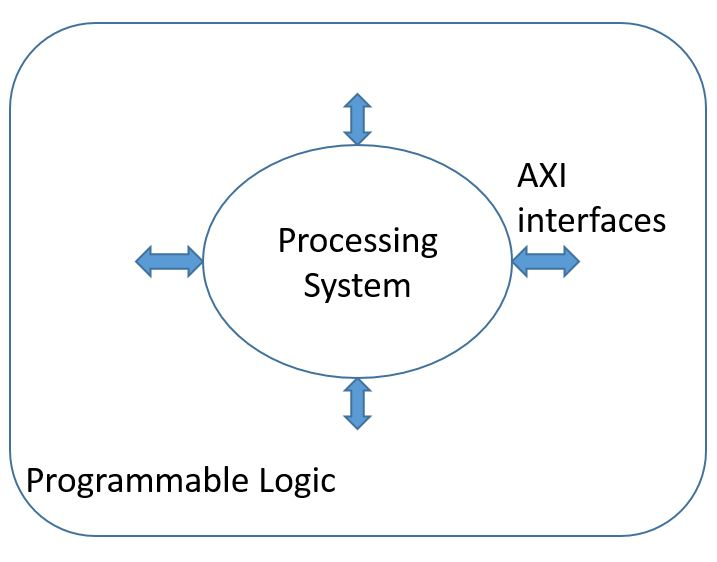
\includegraphics[width = 0.4\textwidth]{media/znyqArch.png}
	\caption{Zynq-7000 Processing System and Programming Logic Architecture}
	\label{fig-zynqProc}
\end{figure}

\section{Hardware Register Interace and Memory-Mapped I/O}
The interface between hardware and software in the Measurement Network Gateway is implemented using memory-mapped registers. This approach provides a well-defined, stable boundary that abstracts low-level hardware details from software while ensuring deterministic access to measurement data and control functions.

\subsubsection{Why we use Registers:}
Registers provide a small, well-defined set of 32-bit memory locations with stable read/write behavior. On the software point of view, each register, each register looks like a simple variable accessible through standard Linux drivers. The FPGA is handling all timing critical operations such as SPI sequencing, ADC conversion control, and GPIO handling. It isolates software from hardware details and allows hardware updates without altering applications.

\subsubsection{Register Structure}
Each register is implemented as a 32-bit word aligned on 32-bit boundaries, ensuring that AXI transactions from the Zynq PS map one-to-one to individual registers without unaligned accesses or partial writes. This simplifies both the Linux driver implementation (MeasObj\_struct with rnum and rvalue fields) and the PL logic that decodes address and data buses.
	
\subsubsection{Read/Write Semantics}
Register behavior is defined per address:

\begin{itemize}
	\item Read-only registers: Status flags, sensor data, GPIO input states
	\item Write-only registers: Control commands, LED outputs, conversion triggers
	\item Command/status registers: Writing initiates hardware action; subsequent reads return completion status or resulting data
\end{itemize}
This contract is captured in the measdif IP core specification and enforced by the /dev/meascdd device driver.

\subsubsection{Synchronization}
The PL updates registers in its own clock domain (typically derived from sensor or AXI clocks), while the PS reads or writes them in the CPU clock domain. The AXI interconnect and internal flip-flop staging ensure that each side sees only fully stable 32-bit values. This hardware-managed synchronization eliminates metastability and timing violations, making the register file the exact point where hardware meets software cleanly. The Linux driver never worries about SPI timing, ADC bit clocks, or clock-domain crossings—it simply reads and writes registers while the FPGA guarantees coherent, time-correct behavior underneath.

\subsection{Linux Device Driver}
The FPGA logic is exposed to the Linux kernel via a custom device driver:
\begin{itemize}
	\item Device file: /dev/meascdd (MEAScdd = Measurement Device)
	\item Type: Character device (read/write registers)
	\item Access method: ioctl() or direct read()/write() calls from C user-space
\end{itemize}
The driver provides memory-mapped register access:

\begin{minted}[bgcolor=lightgray, tabsize = 4, breaklines]{c}
	// Example: Read a status register
	int fd = open("/dev/meascdd", O_RDWR);
	uint32_t reg_value;
	read(fd, &reg_value, sizeof(uint32_t));
\end{minted}
	
\subsection{Hardware-Software Interface}
The boundary between hardware and software in the Measurement Network Gateway is implemented through a custom Linux character device, /dev/meascdd. This device provides a unified interface for accessing all measurement data and digital I/O states. Hardware registers in the programmable logic are mapped into kernel space and exposed to user-space applications through standard file operations.

With this approach, it shields applications from hardware details without losing performance or timing accuracy. Also it is going to simplifies the future modification to hardware, the changing is only effected with the driver part and will not touch or effect on user space software.

\begin{figure}[H]
	\centering 
	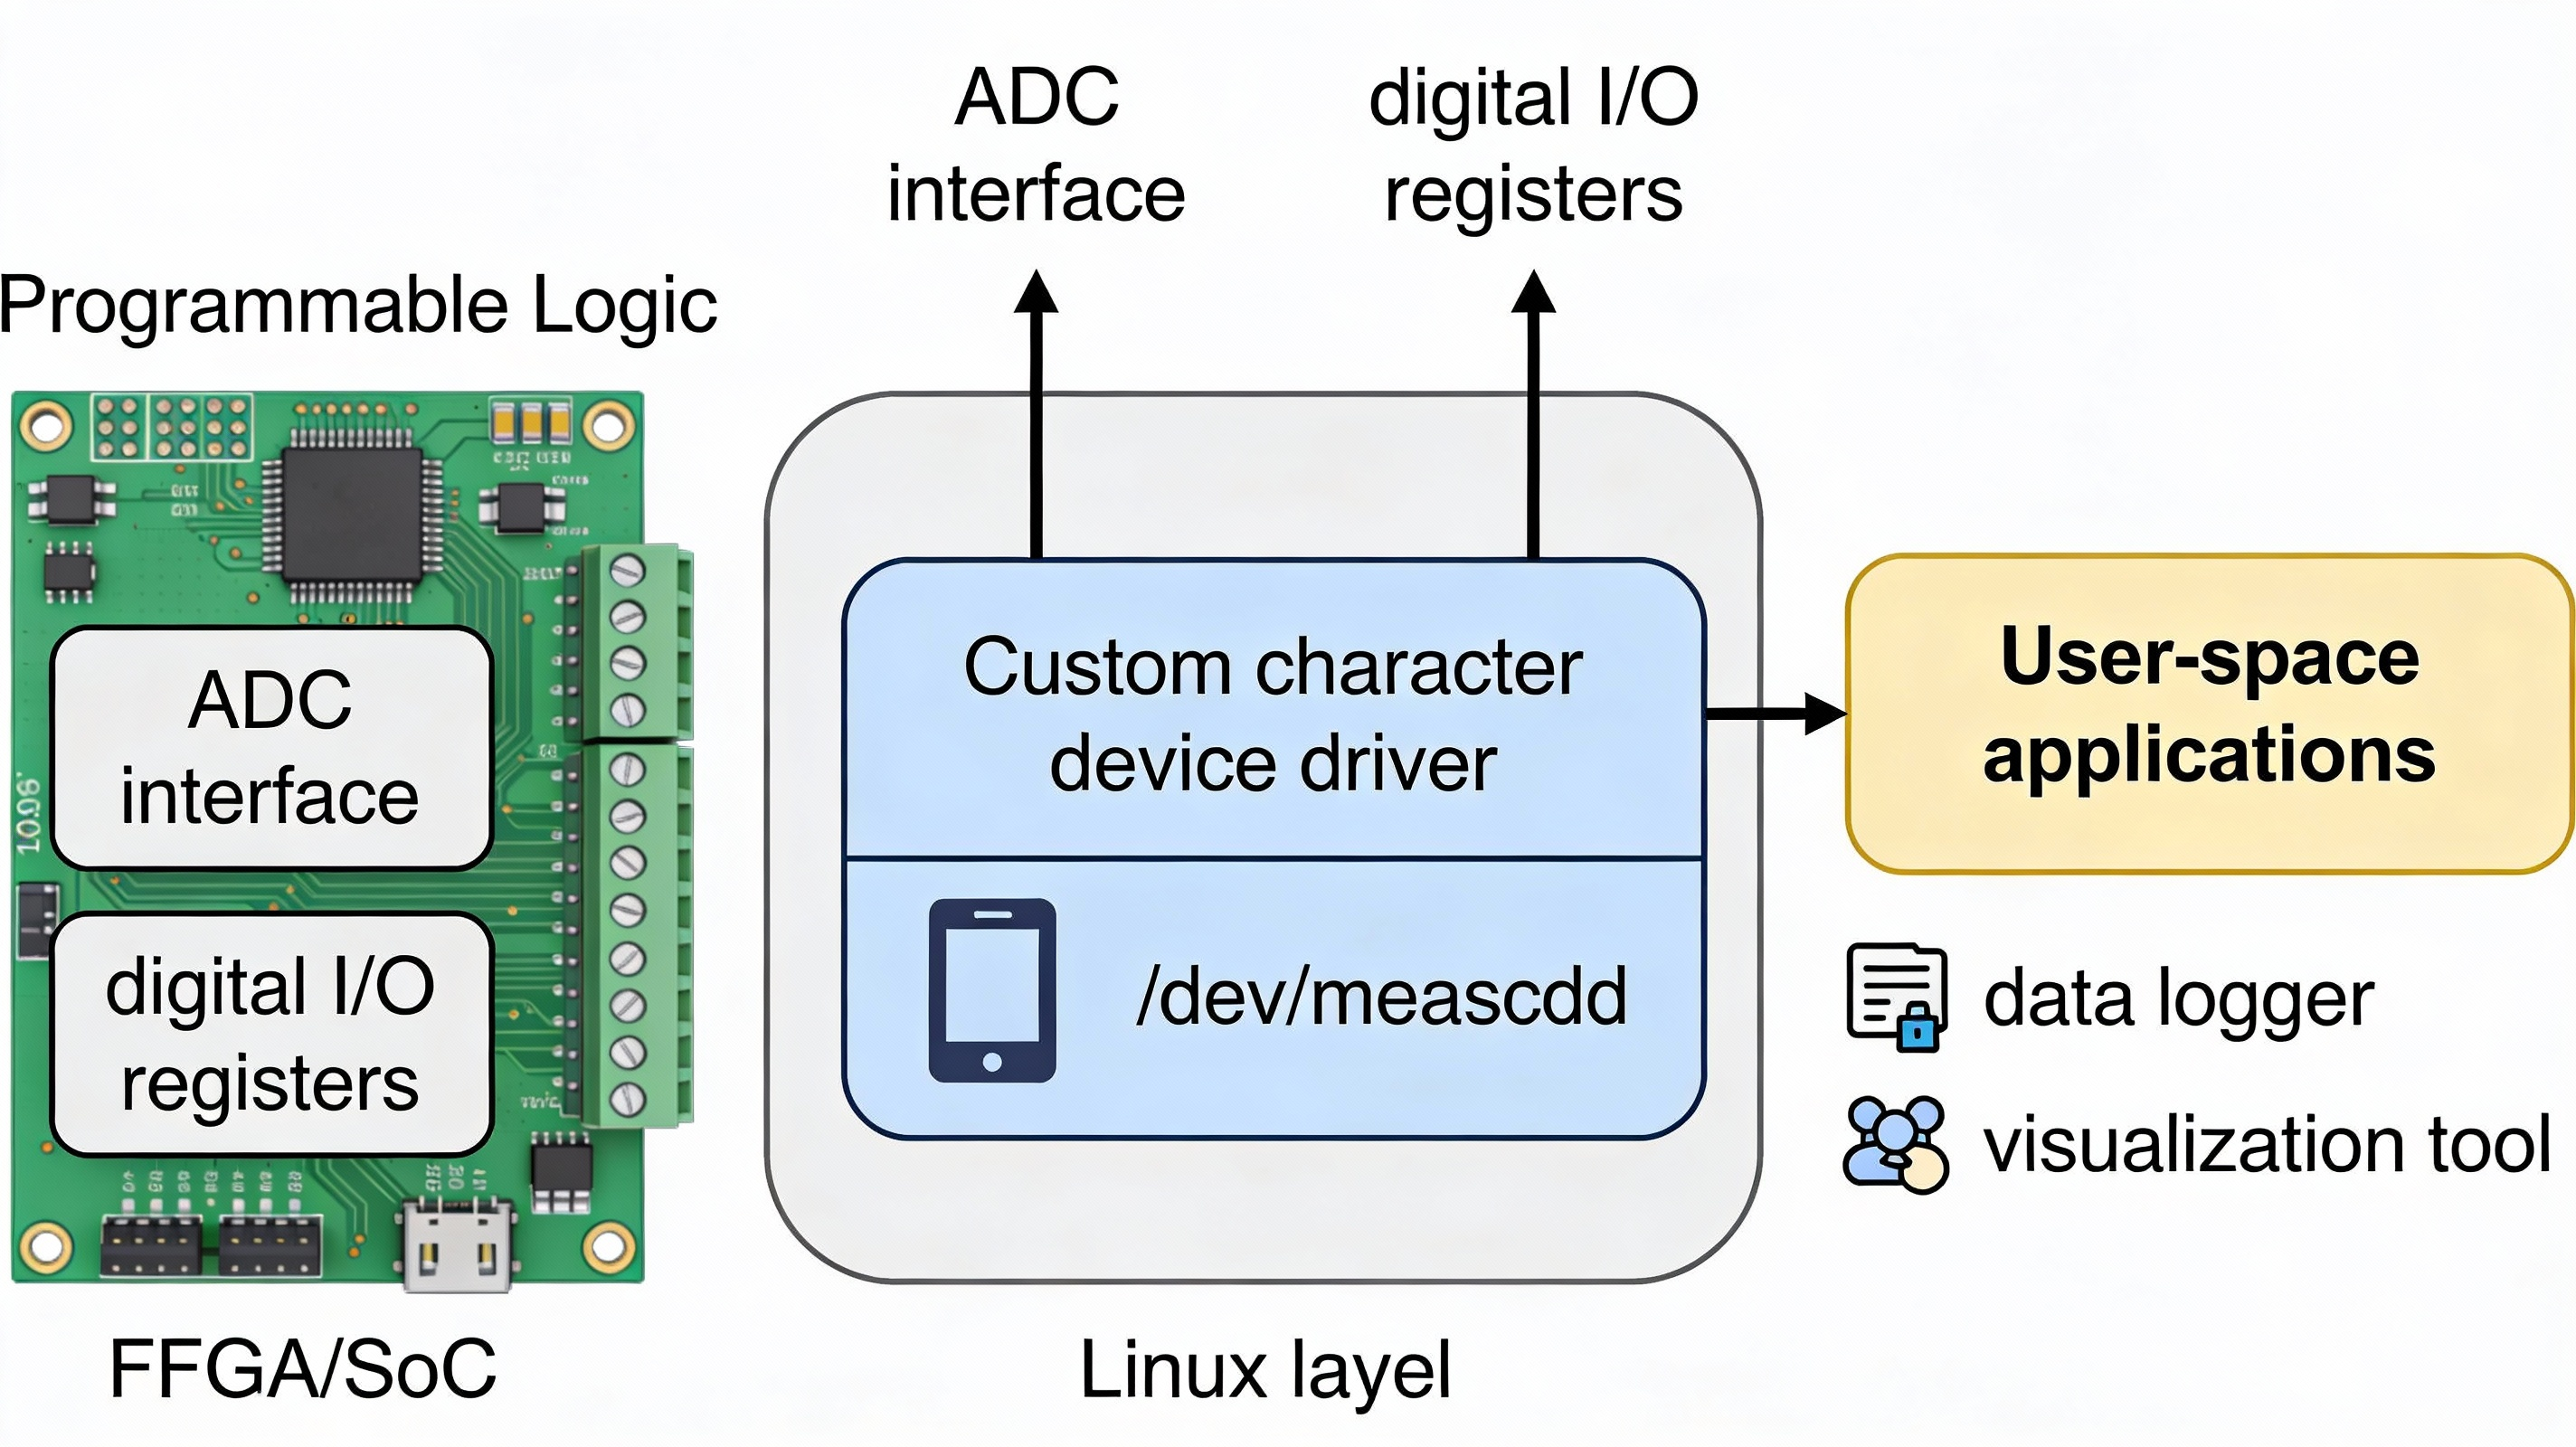
\includegraphics[width = 0.8\textwidth]{media/hard_soft.png}
	\caption{Hardware-Software interface through linux device driver}
	\label{fig-hard-soft}
\end{figure}

\section{Sensor Interface Subsystem}
The Measurement Network Gateway uses dedicated sensor interface subsystems to acquire physical signals and then convert them into reliable digital data, it will be needed for further processing. Each interface provides appropriate excitation, signal conditioning, and protection tailored to the specific sensor type, ensuring accurate and low-noise measurements even in industrial environments. 

\subsection{Temperature Measurement Subsystem}
Temperature measurement plays a key role in this system, because it is needed to monitor the condition of the equipment, apply temperature compensation to other sensors, and maintain safe operating limits in industrial use. For this reason, the gateway contains a dedicated temperature interface that delivers precise, stable temperature data for both laboratory experiments and real world deployments.

\subsubsection{RTD-Based Temperature Measurement}
Temperature measurement in the Measurement Network Gateway is implemented using a platinum Resistance Temperature Detector (RTD), specifically a PT100-type sensor. In the industry and laboratory is mostly used this RTDs because of their high accuracy, excellent long-term stability, and nearly linear resistance–temperature relationship over a wide operating range. If we compare to the semiconductor temperature sensor, it has different behavior. The RTDs provide predictable and repeatable behavior, making them suitable for precise measurements and calibration tasks.

The working principle of this RTDs is based on temperature-dependent resistance of platinum, with increasing of temperature the resistance of RTD element will increase in a good manner. With the correct measurement of the resistance and correctly conversion, the temperature will calculate and determined with high precision. In this project, the RTD serves as the primary sensing element, while all signal excitation, conditioning, and digitization are handled by a dedicated interface IC.

\begin{figure}[H]
	\centering 
	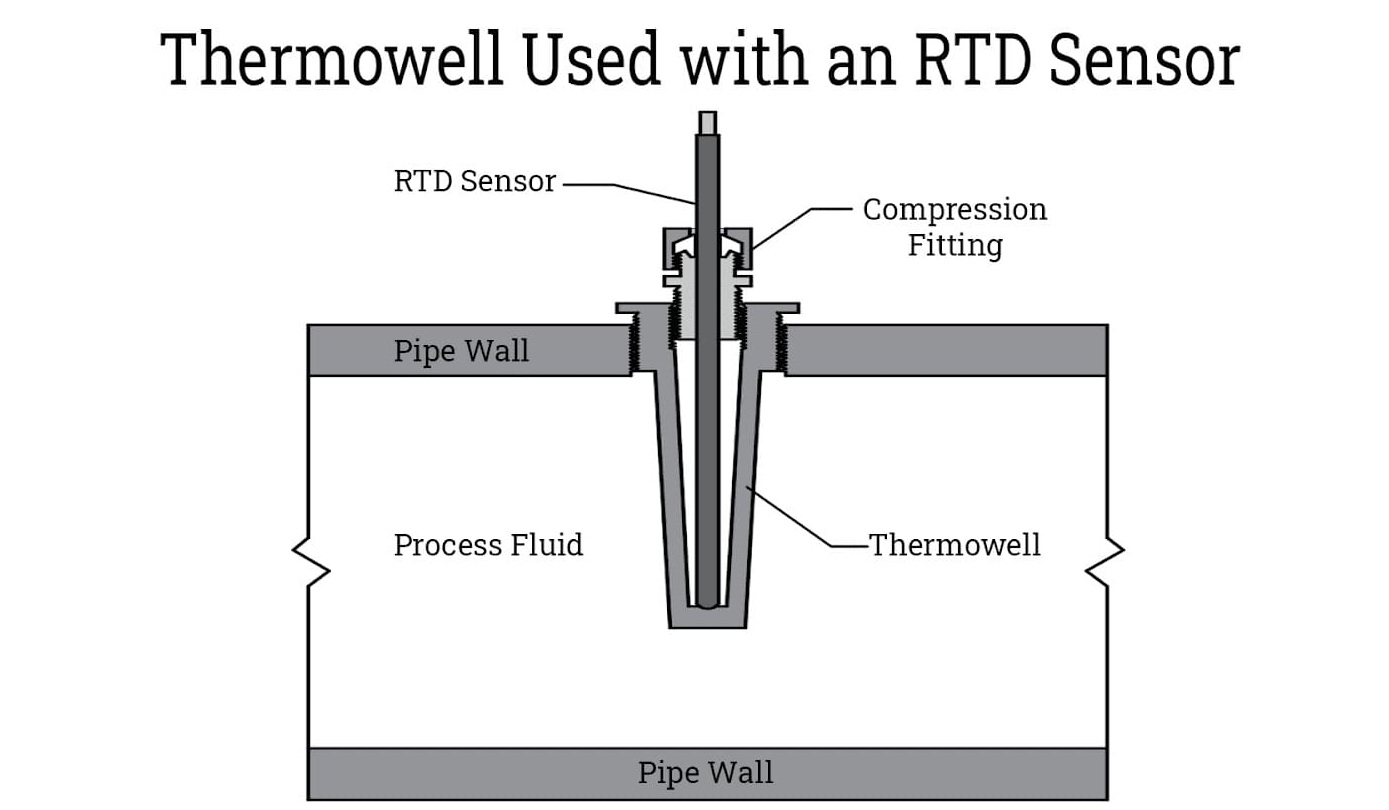
\includegraphics[width = 0.6\textwidth]{media/thrermal.jpg}
	\caption{Thermowell used with an RTD sensor}
	\label{fig-thermowell}
\end{figure}
	
\subsubsection{MAX31865 RTD-to-Digital Converter}
To interface the analog RTD sensor with the digital processing system, the design uses the MAX31865 RTD-to-digital converter. This integrated circuit is specifically designed for precision RTD measurements and significantly simplifies the hardware design. For the RTD, the MAX31865 provides a stable excitation current and measure the voltage drop and converting the resistance value into a digital representation using an internal high resolution analog to digital converter.

The MAX31865 supports multiple RTD wiring configurations, including 2-wire, 3-wire, and 4-wire setups. For our project the jumper setting allow the wiring mode to be selected based on the connected sensor on the module. This device has also the built in fault detection features such as open-circuit, short-circuit, and over-range detection, improving robustness and allowing hardware-level error identification.
The Serial Peripheral Interface (SPI) is a communication path between the MAX31865 and the Zynq platform. During system initialization, configuration registers inside the MAX31865 are programmed to set parameters such as wiring mode, fault detection options, and conversion settings and after the initialization periodic SPI transactions are executed to retrieve the latest conversion results. After initialization, periodic SPI transactions are executed to retrieve the latest conversion results. The achievable update rate is limited by the internal conversion time of the MAX31865 and is typically set to approximately 10 Hz in this project, which is sufficient given the slow dynamics of temperature changes.

Accuracy in this measurement chain is influenced by several factors, including the tolerance class of the RTD sensor, the reference resistor used by the MAX31865, ADC resolution, and PCB layout. Under typical laboratory conditions and with basic calibration, the system achieves temperature accuracy on the order of a few tenths of a degree Celsius to approximately ±1 °C. Environmental effects such as lead resistance and RTD self-heating are also relevant; long or thin wires increase series resistance, and excessive excitation current can slightly warm the sensor. These factors are mitigated through appropriate wiring configuration and conservative excitation settings.

\begin{figure}[H]
	\centering 
	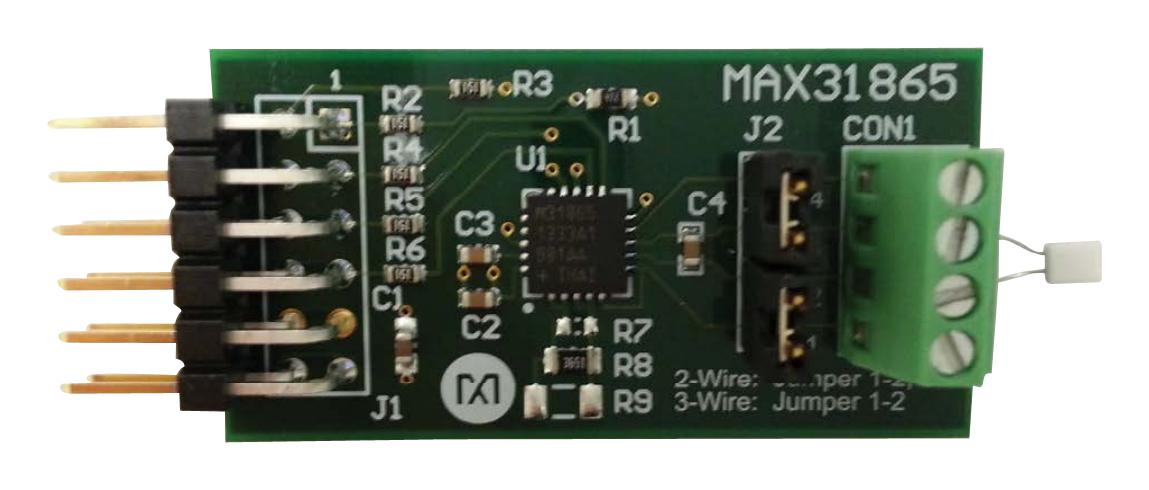
\includegraphics[width = 0.6\textwidth]{media/rtd.jpg}
	\caption{MAX31865 module with connected RTD sensor}
	\label{fig-rtd}
\end{figure}
	
	
\subsubsection{Integration into the Measurement System}
The temperature measurement subsystem is tightly integrated into the overall Measurement Network Gateway architecture through the programmable logic of the Zynq-7000 SoC. The FPGA-based programmable logic implements the SPI master that communicates with the MAX31865, ensuring precise timing and deterministic control of the SPI clock, chip select, and data signals. When a temperature conversion is complete, the programmable logic retrieves the digital result and stores it in memory-mapped registers connected to the AXI interconnect.

These registers are exposed to the processing system through the custom measdif hardware interface and accessed in software via the /dev/meascdd Linux character device. The user-space measurement application periodically reads the temperature registers, associates each value with a timestamp and a unique sensor identifier, and inserts the data into the shared ring buffer. From there, the measurements are forwarded to the network subsystem and transmitted to the remote graphical user interface.

This hardware–software partitioning ensures that all time-critical tasks, including SPI timing, conversion control, and data latching, are handled deterministically in hardware, while higher-level tasks such as buffering, networking, and visualization are managed in software. The result is a robust, accurate, and industry-relevant temperature measurement solution that integrates cleanly into the overall gateway architecture.

\begin{table}[H]
	\centering 
	\begin{tabularx}{\textwidth}{|X|X|}
		\hline 
		\textbf{Parameter} & \textbf{Value} \\ \hline 
		RTD Type & PT100 \\ 
		Update Rate & $\approx \SI{10}{\hertz}$ \\ 
		Typical Accuracy & $\pm\ 0.5$ to $\pm \SI{1.0}{\degreeCelsius}$ (Uncalibrated) \\ 
		Interface & SPI via MAX3865 \\ \hline 
	\end{tabularx}
	\caption{Key Specification of the RTD-Based temperature Measuremnt}
\end{table}

\subsection{Analog Data Acquisition Subsystem}
The analog data acquisition subsystem converts the low-level analog signals into the precise digital values which is processed by the FPGA and embedded software. It is going to provide the required input range, resolution, and sampling performance to capture slow- and medium-speed sensor signals without distortion, when it ensures stable and repeatable measurements through proper interfacing and timing control.

\subsubsection{PmodAD1 Analog-to-Digital Converter}
The PmodeAD1 module which is responsible for the measurement of  analog voltage in this project and PmodAD1 integrates two Analog Devices AD7476A 12-bit successive-approximation ADCs which provide two independent single-ended analog input channels. Each converter operates over a voltage range of approximately 0 V to 3.3 V, referenced to the ZedBoard’s analog supply.

The chip select and serial clock which are the control signal, and also the data transfer on the MISO line are generated and handled by the programmable logic. This hardware-driven SPI implementation ensures deterministic sampling behavior and avoids timing jitter associated with software-controlled I/O.

Mechanically and electrically, the PmodAD1 is connected to the ZedBoard through the JA1 Pmod header. The 2×6 pin Pmod connector directly maps FPGA I/O pins to the ADC control and data signals, allowing low-latency and tightly synchronized communication between the ADC and the FPGA fabric.

\begin{figure}[H]
	\centering 
	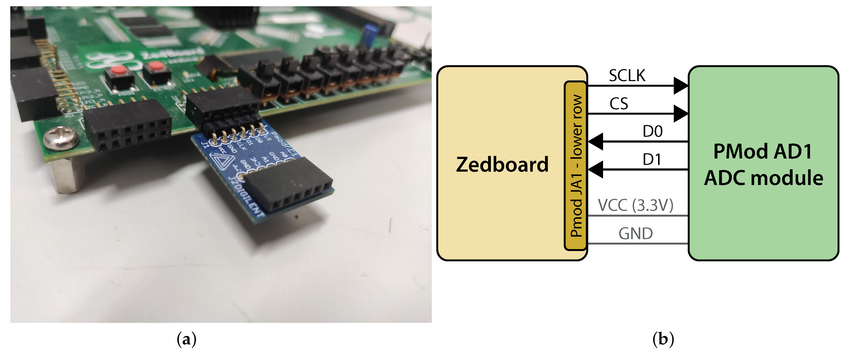
\includegraphics[width = 0.6\textwidth]{media/pmod.png}
	\caption{PmodAD1 module mounted on the Zedboard}
	\label{fig-pmod}
\end{figure}

\textbf{Specification:}
\begin{table}[h]
	\centering
	\caption{ADC Specifications}
	\begin{tabular}{ll}
		\toprule
		\textbf{Parameter} & \textbf{Value} \\
		\midrule
		Resolution & 12 bits \\
		Number of Channels & 2 (A0, A1) \\
		Input Range & 0 to 3.3\,V (configurable) \\
		Sampling Rate & Programmable via software \\
		Interface & SPI (MOSI, MISO, CLK, CS) \\
		Supply Voltage & 3.3\,V (from ZedBoard) \\
		\bottomrule
	\end{tabular}
	\caption{PmodAD1 Analog-to-Digital Converter Specification}
\end{table}

\subsubsection{Signal Acquisition and Conversion Characteristics}
External analog signals are supplied using laboratory equipment such as a function generator. And these all signals are applied through the PmodAD1 analog input channels. While the operation, the programmable logic is going to initiates SPI transaction at the chosen sampling rate, starts ADC conversions, and reads the digital values.

Each AD7476A produces a 12-bit value between 0 and 4095 for the full-scale input range. With a 0–3.3 V range, each LSB represents roughly 0.8 mV. The ideal quantization error is therefore ±0.5 LSB, although practical measurements also include additional uncertainty due to ADC offset, gain error, reference voltage stability, and noise.

The ADC reference voltage is derived from the ZedBoard’s regulated 3.3 V rail. As a result, any ripple or drift on this supply directly affects conversion accuracy. The clock derived from the FPGA fabric is responsible for sampling timing and the stability of this clock ensures consistent sampling intervals and minimizes timing jitter, which is particularly important when observing dynamic signals such as sine waves.

\begin{figure}[H]
	\centering 
	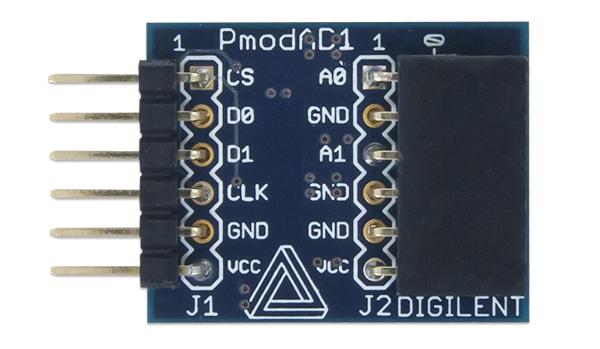
\includegraphics[width = 0.3\textwidth]{media/pmod2.png}
	\caption{Analog data acquisition using PmodAD1}
	\label{fig-pmod2}
\end{figure}

\subsection{Digital Input and Output Interfaces}
The digital input and output interfaces of the Measurement Network Gateway is going to provide the main means for user interaction and simple control signaling. They connect board-level switches, pushbuttons, and GPIO signals to the programmable logic, it is enabling the manual test inputs, status indication, and coordination with external devices.  With the exposing of these signals through memory-mapped registers and Linux drivers, the system allows software to monitor and control digital I/O flexibly and reliably.


\subsubsection{Switches and PushButtons}
The ZedBoard includes user-accessible switches and pushbuttons connected to the programmable logic through GPIO interfaces. These inputs operate at 3.3 V logic levels and are buffered by on-board circuits that include fixed pull-up or pull-down resistors to ensure defined logic states when switches are open. Logic '1' and '0' correspond to 3.3 V and 0 V at the FPGA input pins, as defined by the ZedBoard schematic and FPGA pin constraints.

Debouncing is handled primarily in software. The sensor layer samples GPIO states at a moderate rate (typically tens of Hz), and brief contact bounce is either filtered by this sampling interval or can be ignored for the measurement use case. No additional RC networks or Schmitt-trigger circuits were required, as the ZedBoard's user I/O already provides adequate buffering and signal conditioning.
The digital state of all switches and pushbuttons is read by the FPGA and stored in memory-mapped GPIO input registers. The Linux device driver exposes these values to user-space software, allowing the measurement application to monitor user interactions and use them for testing, debugging, or basic control functions.

\subsubsection{LEDs}
User LEDs on the ZedBoard are controlled through GPIO output registers implemented in the programmable logic. Each LED is driven from an FPGA output pin through an on-board series current-limiting resistor that restricts current to a few milliamps. This current level is safe for the FPGA I/O and provides sufficient brightness for clear visual indication.

The measurement application uses the LEDs to provide real-time visual feedback. For example, LED states can mirror the current position of input switches, indicate active sampling, or signal connection status. Because the current-limiting resistors are already present on the board, the software can safely write switch bits directly to LED outputs without risk of over-current.

\begin{figure}[H]
	\centering 
	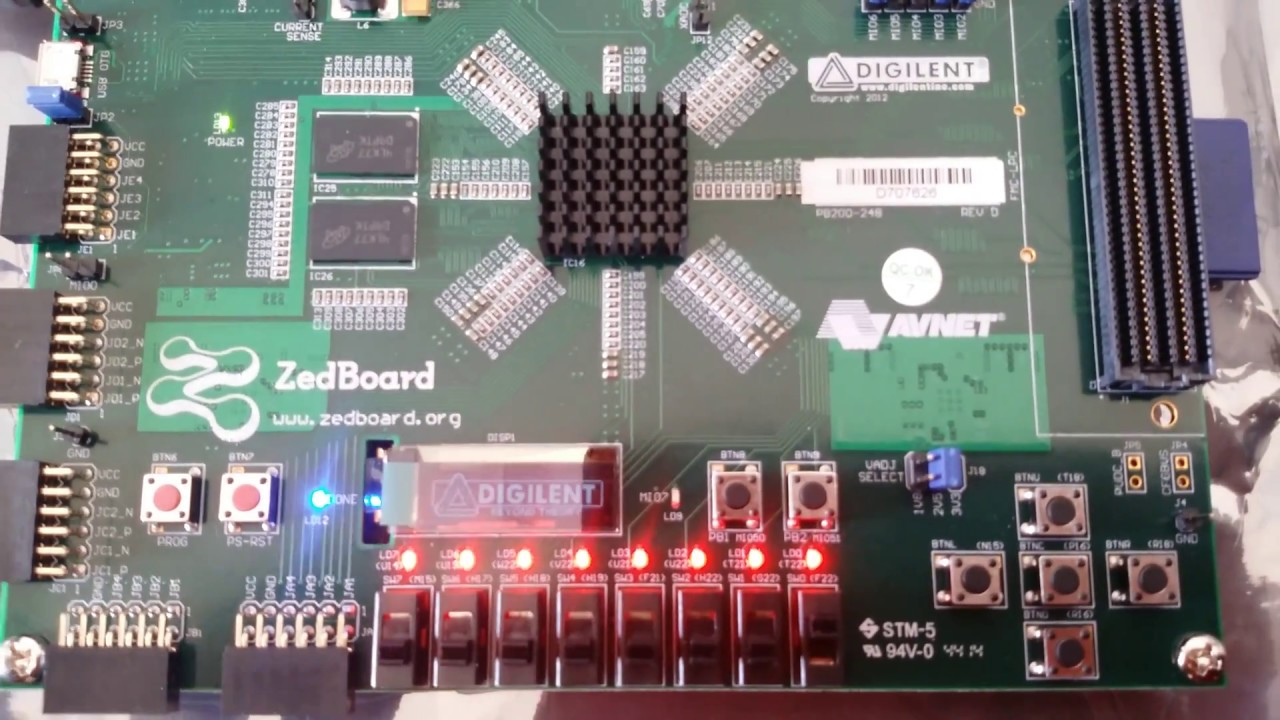
\includegraphics[width = 0.6\textwidth]{media/leds.jpg}
	\caption{ZedBoard user interface showing switches and LEDs in operation}
	\label{fig-leds}
\end{figure}

\subsubsection{Ethernet and Network Interface}
The Measurement Network Gateway uses the integrated Ethernet interface of the Zynq processing system to communicate with external clients. The external PHY connection which the Ethernet controller connected to that, it is providing a standard RJ45 interface. It allows the system directly connect to a local network or a single host computer for that hardware configuration

The Ethernet interface enables the transmission of measurement data using TCP/IP, providing reliable and ordered data delivery. The use of standard networking protocols ensures compatibility with a wide range of client systems.
\begin{figure}[H]
	\centering 
	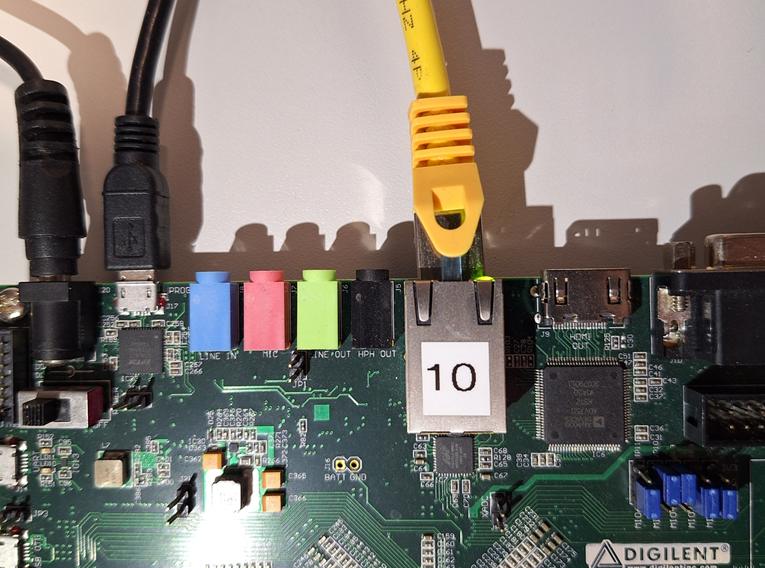
\includegraphics[width = 0.6\textwidth]{media/ethernet.png}
	\caption{Ethernet Connection between the Zedboard and host PC}
	\label{fig-ehternet}
\end{figure}

\section{Timing, Interrupts and Hardware synchronization}
Reliable and deterministic timing is a fundamental requirement of the Measurement Network Gateway, as multiple sensors must be sampled at well-defined intervals while operating within a Linux-based environment. To avoid the nondeterministic behavior associated with software-based delays, all timing-critical operations are implemented in hardware inside the programmable logic (PL) of the Zynq device. Interrupts and status signaling mechanisms are then used to synchronize these hardware events with the processing system (PS).

\subsection{Hardware Timing Sources}
Timing events in the system are generated by clocked hardware implemented in the programmable logic. A base fabric clock (for example 100 MHz) is divided down using counters and clock-enable logic to create slower, application-specific timing signals. These timing signals set the controlling ADC sampling intervals, MAX31865 temperature conversion cycles, and GPIO sampling rates.

Each hardware timing logic is responsible for the its own sensor interface and it ensures the sampling occurs at precise and repeatable intervals independent of the Linux scheduler. This approach guarantees deterministic sampling behavior and allows multiple sensors to operate concurrently at different configured frequencies.

\subsection{Interrupt and Event Handling}
When a sensor conversion or measurement cycle completes, the programmable logic sets dedicated status bits in memory-mapped registers exposed through the measurement interface. Examples include “ADC done” or “MAX31865 conversion complete” flags. The processing system monitors these events either by polling the status registers or, in a more advanced configuration, through hardware interrupts.

Interrupts allow the ARM processor to remain idle or perform other tasks instead of continuously polling registers. When an interrupt is asserted from the PL to the PS, the Zynq Generic Interrupt Controller (GIC) wakes the processor, which then reads the corresponding data and status registers, stores the sample into the ring buffer, and resumes normal operation. This mechanism improves CPU efficiency while maintaining fast response times.

\subsection{Synchronization Strategy}
Synchronization between sensor sampling and software processing is achieved through a combination of hardware-controlled timing and software-level timestamping. Because the sampling instants are defined by hardware clocks in the PL, the timing of each measurement is stable and predictable. When the processing system retrieves a sample, it associates it with an elapsed-time or timestamp value to preserve temporal ordering.

If interrupts are missed due to masking, overload, or software faults, the hardware continues sampling at the correct rate, but samples may remain unread in registers or be overwritten by newer data. This can result in dropped measurements or stale data. To mitigate this risk, the software includes timeout checks and buffer management mechanisms to detect abnormal conditions and apply corrective actions, such as reporting errors or reducing sampling frequency.

\section{Measurement and Validation Equipment}
Validation of the Measurement Network Gateway hardware is performed using standard laboratory measurement equipment to observe signals at different points along the measurement chain. The objective of this validation is to confirm correct electrical behavior, timing integrity, and correspondence between physical signals and digital measurement results produced by the system.

The validation process focuses on three main areas: analog signal integrity at the sensor inputs, correct operation of digital communication interfaces such as SPI, and consistency between measured values and trusted reference instruments.

\begin{figure}[H]
	\centering 
	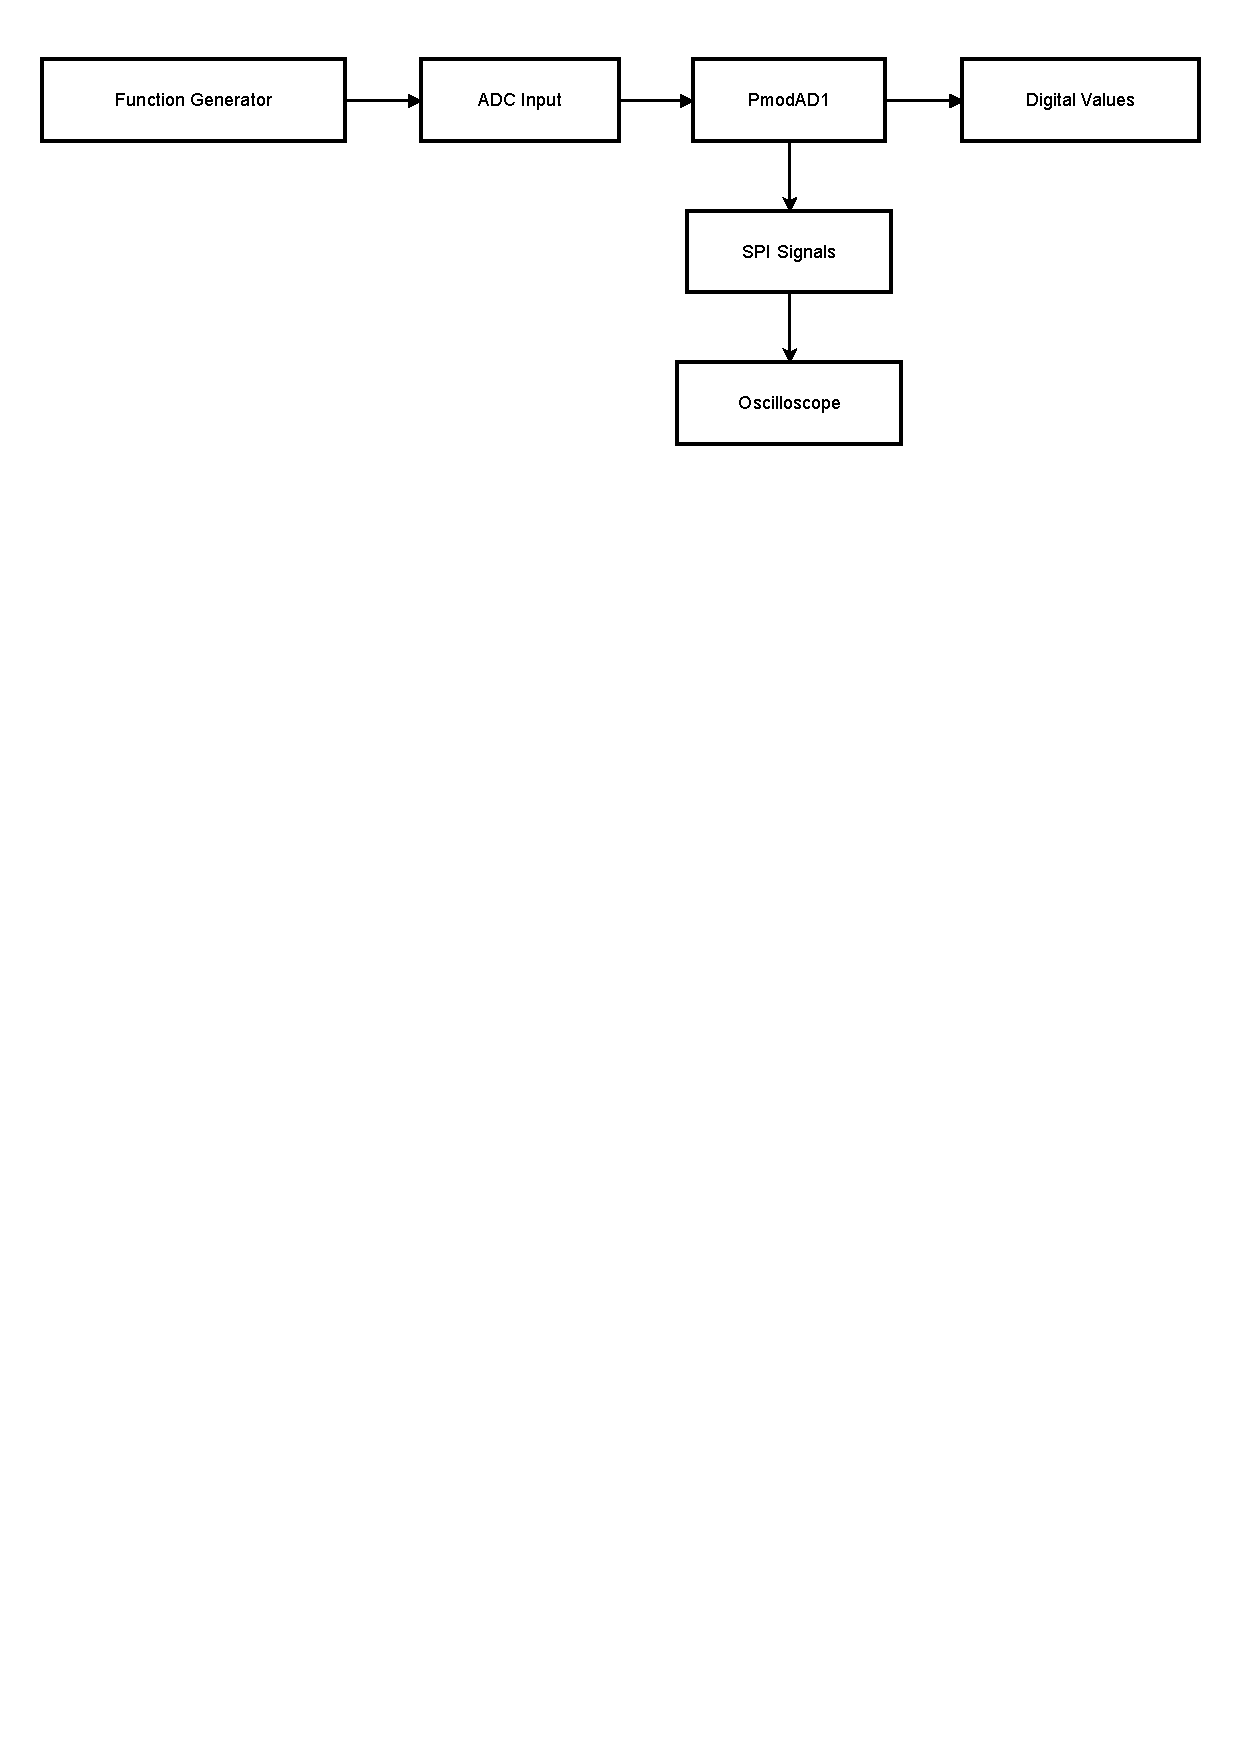
\includegraphics[width = 0.9\textwidth, trim = 0cm 22cm 0cm 0cm, clip]{media/validation.pdf}
	\caption{Validation Measurement Point}
	\label{fig-validation}
\end{figure}

\subsection{Validation Methodology}
During validation, external instruments are used to generate known input signals and to observe internal hardware signals. For the ADC subsystem, a function generator provides controlled DC or sinusoidal voltages to the PmodAD1 inputs. These signals are monitored directly using an oscilloscope and multimeter, while the corresponding digital output values are read from the gateway.

SPI communication between the Zynq programmable logic and peripheral devices such as the PmodAD1 ADC and MAX31865 temperature sensor is examined by probing the clock, chip-select, and data lines. Correct operation is indicated by stable clock frequency, clean chip-select timing, and consistent data transitions synchronized with the clock edges.

Fault conditions can be identified by characteristic symptoms, including distorted or clipped analog waveforms, missing or irregular SPI clock pulses, static data lines despite changing inputs, excessive noise or jitter in ADC codes, or systematic offset and gain errors compared with reference measurements.

\subsection{Laboratory setup and Reference Equipment}
The validation setup uses standard laboratory instruments to provide controlled inputs, stable power, and accurate reference measurements. These instruments allow both static and dynamic verification of the measurement chain and ensure repeatable test conditions.

Key equipment includes:
\begin{itemize}
	\item Function generator for analog input signals
	\item Regulated laboratory power supplies
	\item Digital multimeter for reference voltage and current measurements
	\item Digital storage oscilloscope for timing and signal integrity analysis
\end{itemize}

\subsection{Hameg Triple Power Supply and Digital Multimeter}
It is one of the power supply which is used for the stable and low noise DC power to the ZedBoard, sensor modules, and auxiliary circuits. It has multiple independent and different outputs which allow different subsystems to be to be powered and tested under controlled conditions, while adjustable voltage levels and current limiting protect the hardware during experimentation. 

For the reference instrument of static electrical measurement used the HM8011-3 digital multimeter which provide high resolution readings of voltage and current, enabling precise monitoring of supply rails, sensor excitation voltages, and calibration points. By comparing these reference measurements with the digital values reported by the gateway’s ADC subsystem, offset errors, gain errors, and overall measurement accuracy can be evaluated.
\begin{figure}[H]
	\centering 
	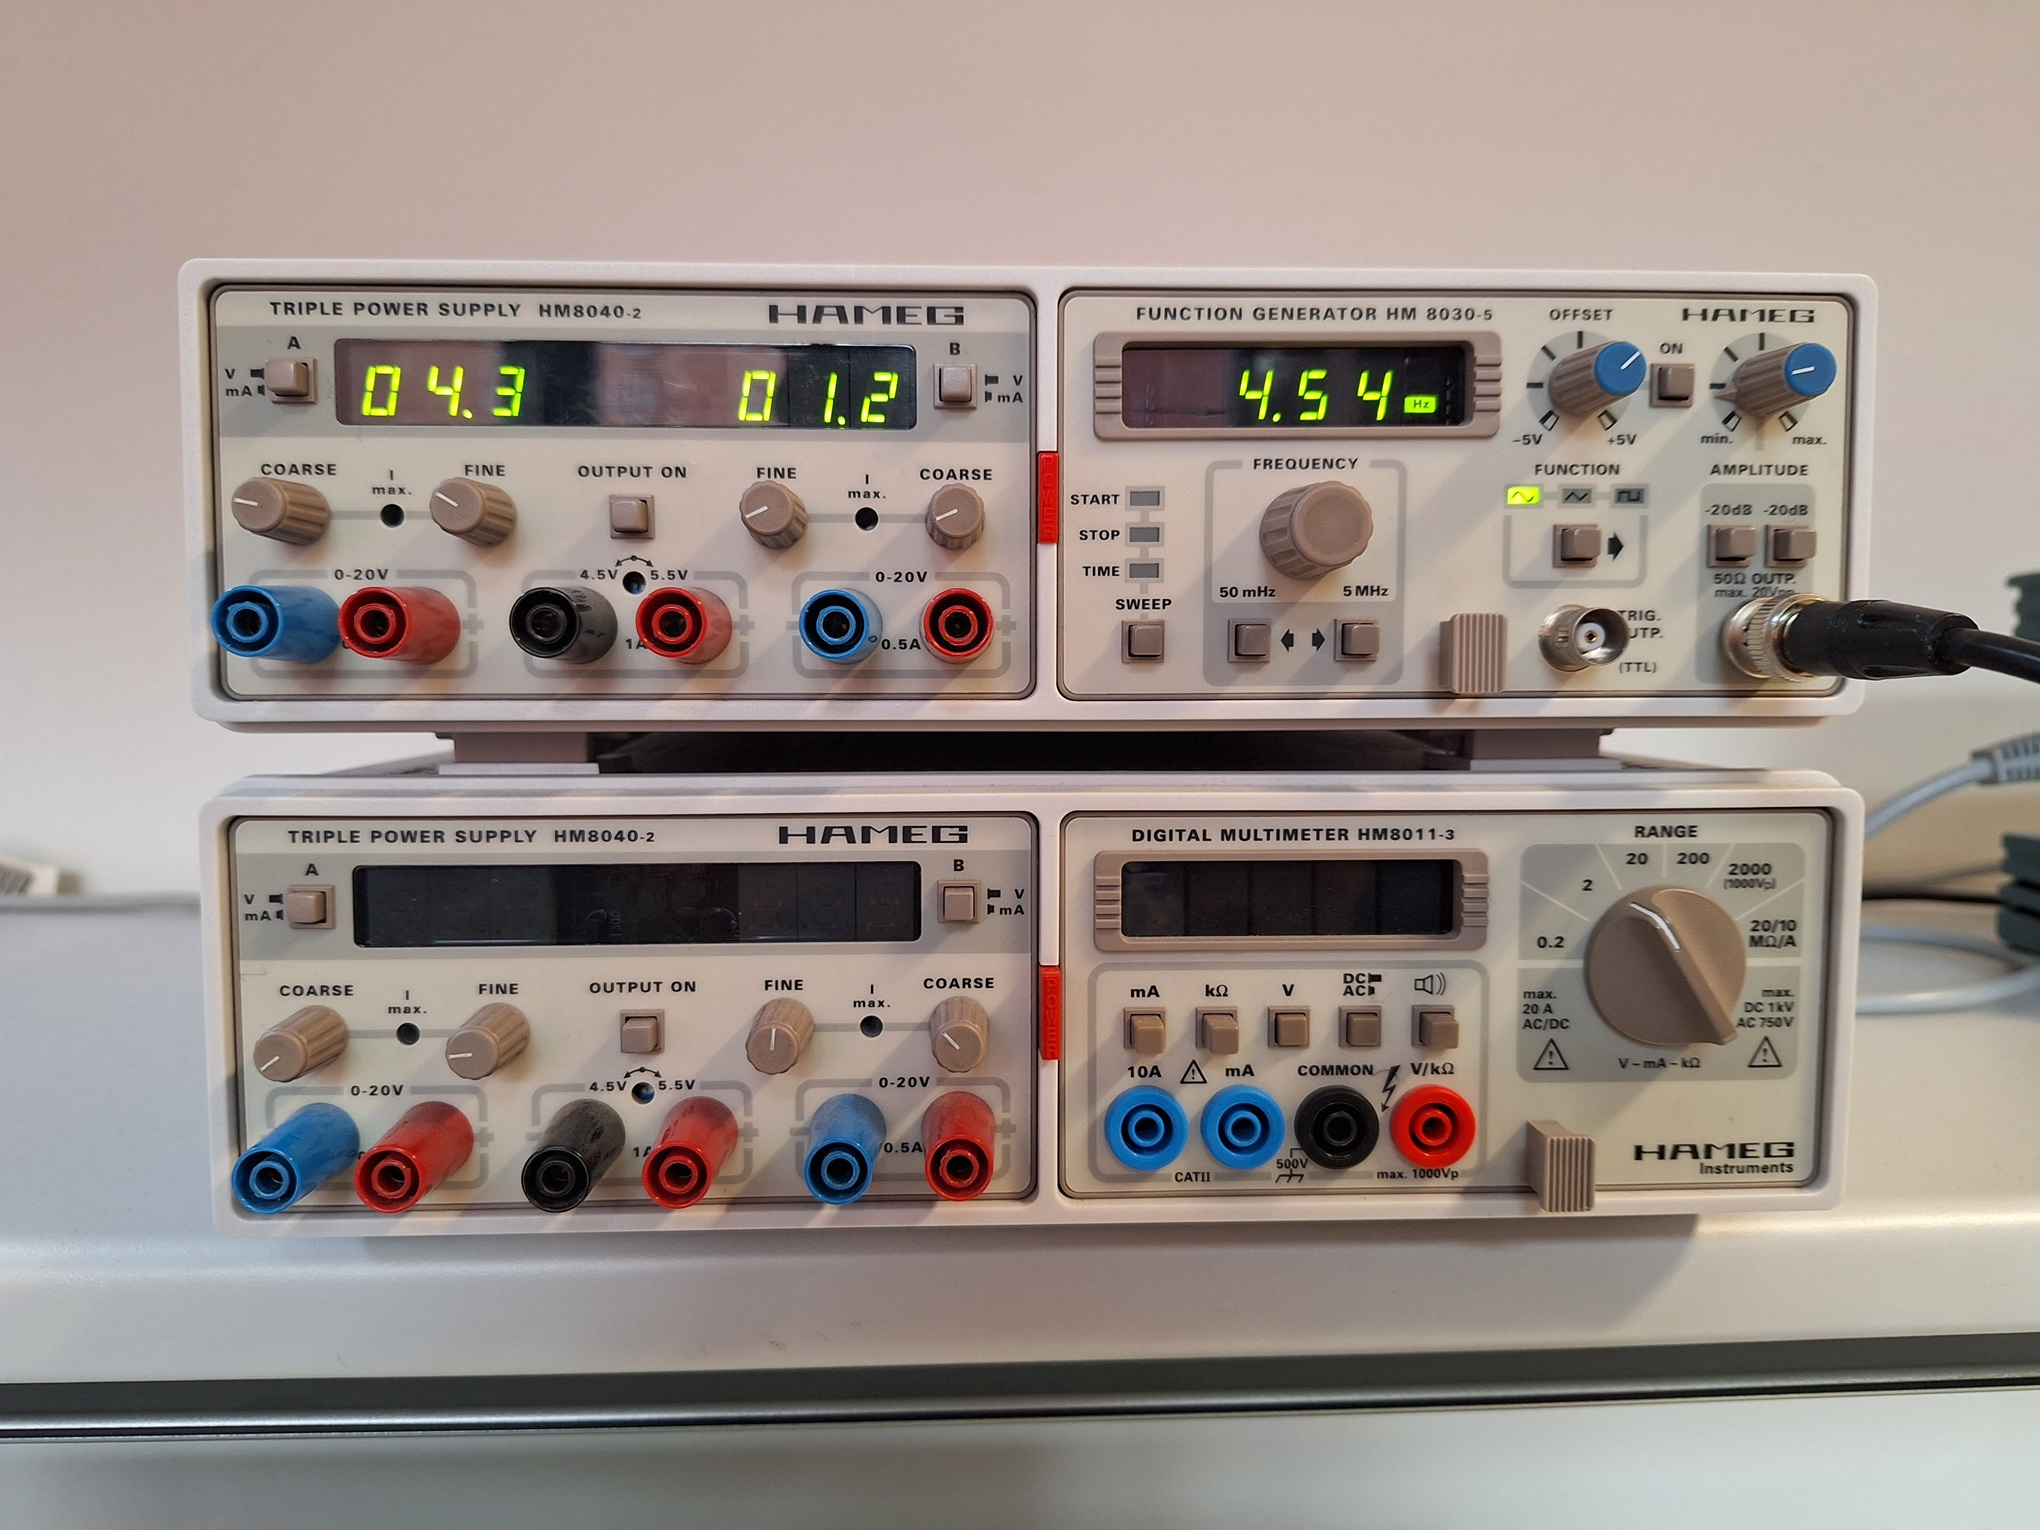
\includegraphics[width = \textwidth]{media/ocsi.jpg}
	\caption{Hameg power supply and multimeter used for power delivery and reference measurements}
	\label{fig-ocsi}
\end{figure}

\subsection{Tektronix TDS2014B Digital Storage Oscilloscope}
The Tektronix TDS2014B digital storage oscilloscope is used to analyze the dynamic behavior of both analog and digital signals within the system. Its four-channel input, 100 MHz bandwidth, and real-time sampling capability of up to 1 GS/s allow simultaneous observation of multiple signals.

Typical measurements include the analog input waveform applied to the ADC, the SPI clock and chip-select signals, and the serial data lines. Time-domain analysis is used to verify waveform shape, amplitude, and timing relationships, while triggering and automated measurements assist in checking setup and hold times and identifying potential timing violations.

The oscilloscope’s FFT capability is also used to assess noise and harmonic content in analog signals. This makes it possible to correlate observed noise or distortion in the digital measurement results with physical effects on the analog input or communication lines.

\begin{figure}[H]
	\centering 
	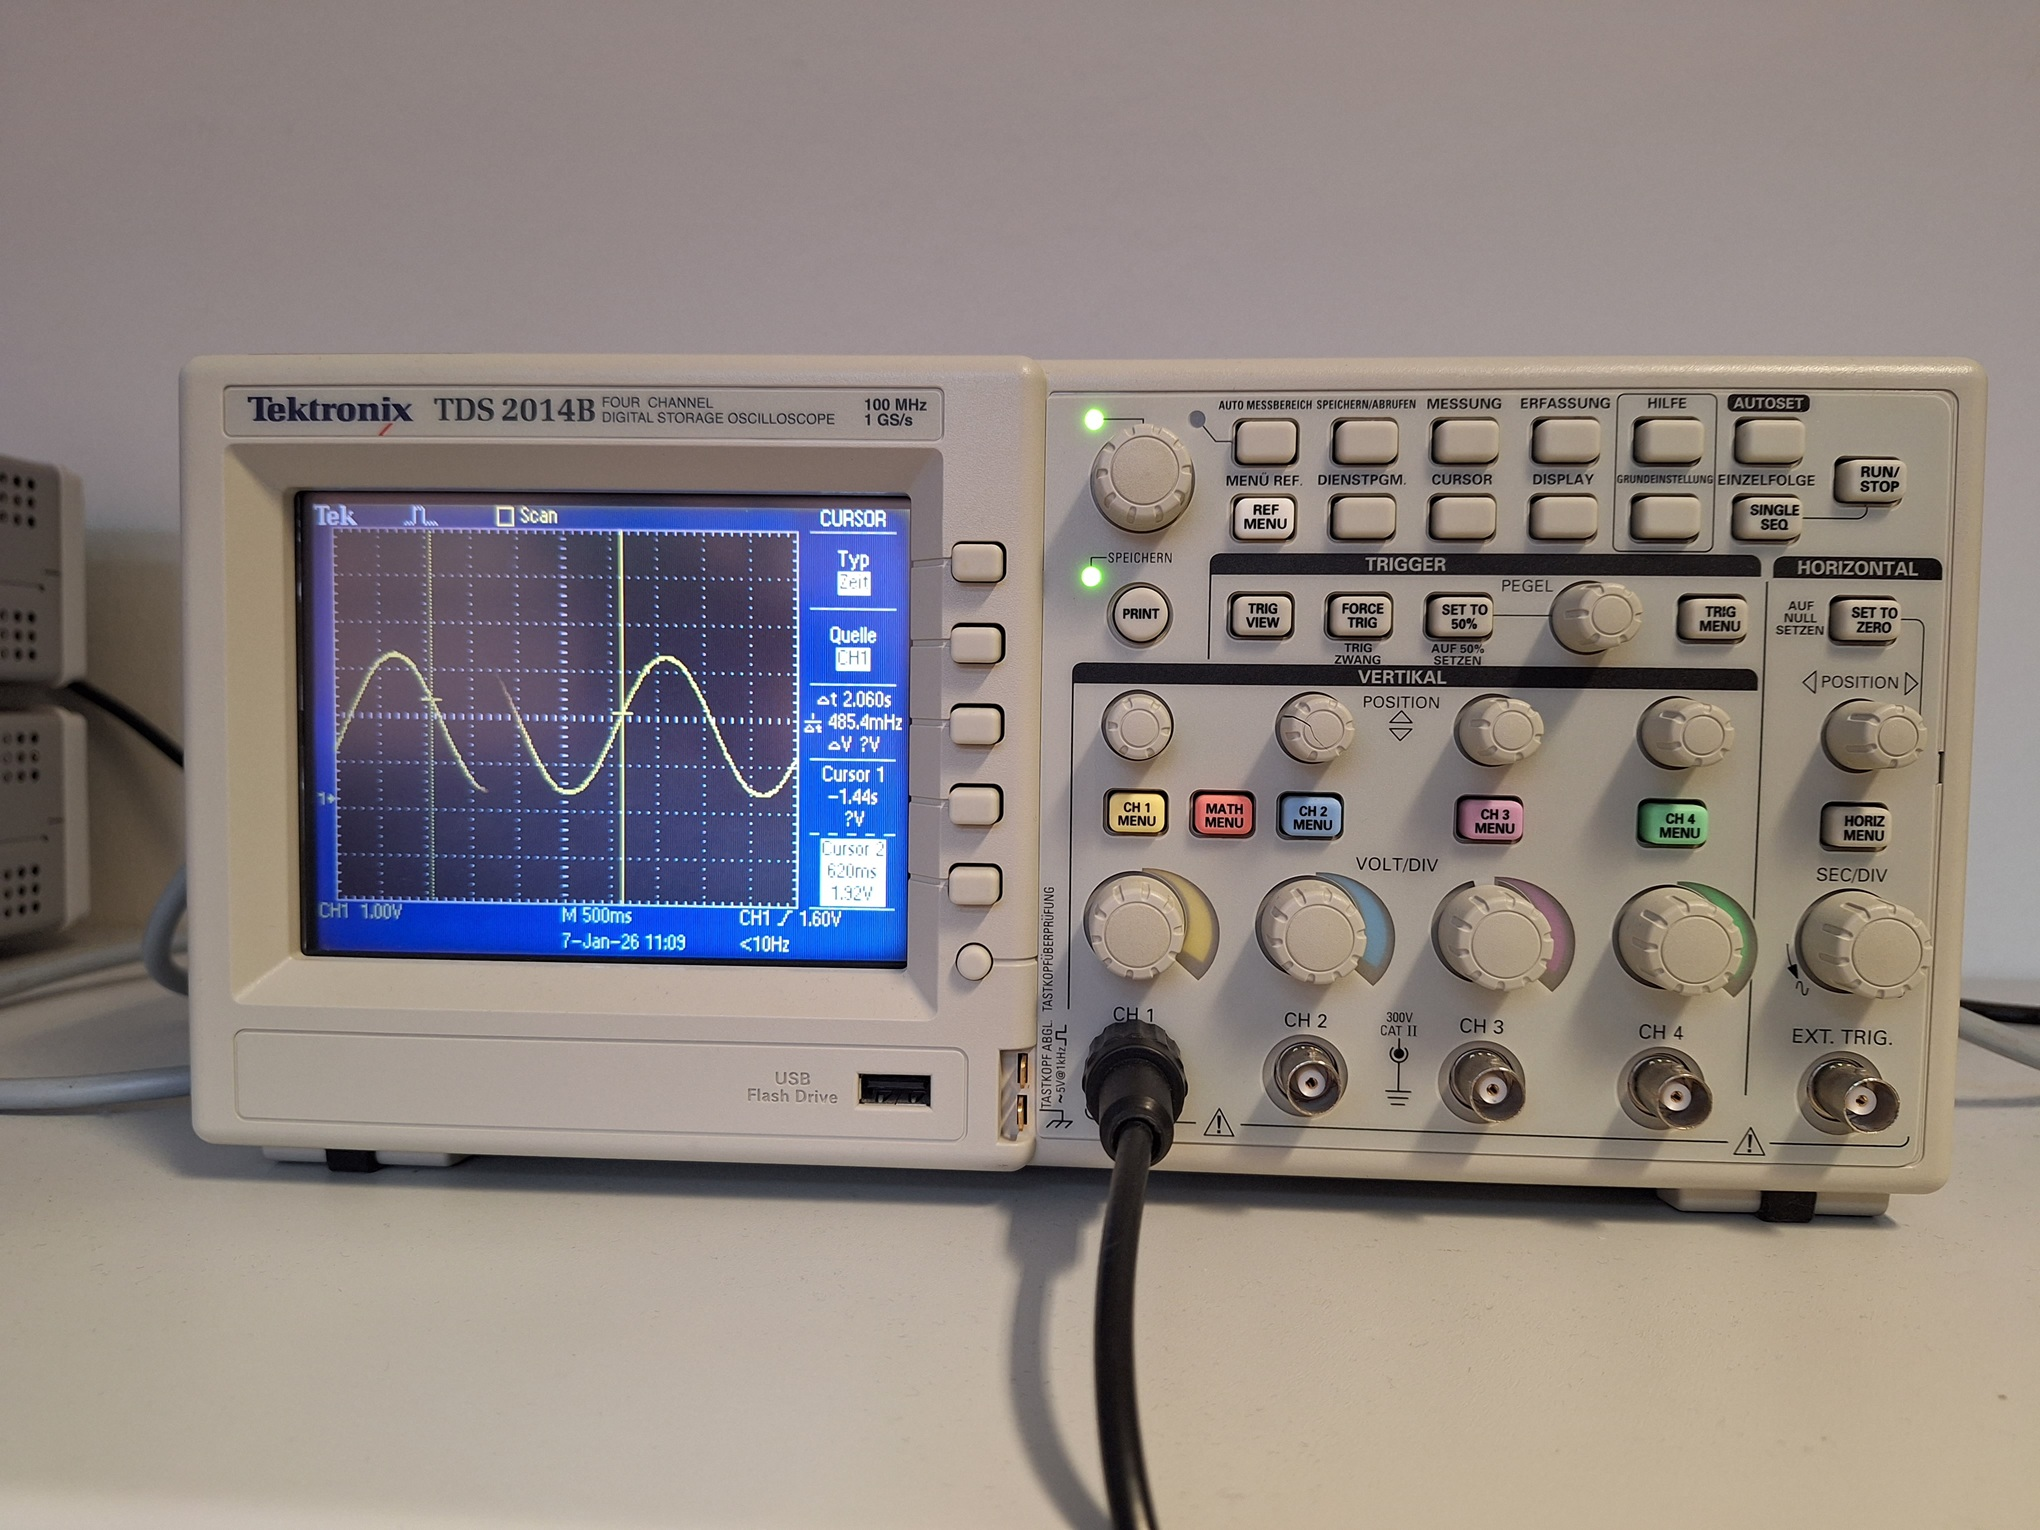
\includegraphics[width = \textwidth]{media/func.jpg}
	\caption{Oscilloscope measurement of SPI timing during ADC conversion.}
	\label{fig-func}
\end{figure}

\subsection{Discussion and Design Considerations}
The measurement and validation results confirm that the hardware design meets its intended functional requirements under laboratory conditions. The FPGA based timing control with combination of Linux based processing will provide reliable operation while keeping hardware complexity manageable.

The Validation of system is being simplifies with the modular structure which can act as individual subsystem for testing independently before being integrated. While the current setup is suitable for educational and general-purpose laboratory measurements, the validation process also highlights areas where additional filtering, shielding, or isolation would be required for high-precision or industrial applications.

\section{Hardware Safety, Reliability, and Robustness}
The hardware platform of the Measurement Network Gateway is designed with fundamental safety and robustness features which is suitable for laboratory and educational environments. It relies on low-voltage signal levels, which is integrated protection features of the ZedBoard, and also deterministic FPGA-based control to reduce the risk of damage, unsafe conditions, or unexpected behavior during normal operation. Together, these measures provide an appropriate level of electrical safety and reliability for the intended environment, which is allowing additional external protections to be added for harsher industrial deployments.

\subsection{Electrical Safety}
The hardware design operates entirely within low-voltage domains suitable for laboratory and educational use. All sensor interfaces, including the PmodAD1 ADC inputs and the MAX31865 RTD interface, operate at 3.3 V logic levels, which are safely supported by the ZedBoard and its FPGA I/O banks. RTD sensor wiring carries only low-level excitation currents and voltages, ensuring no exposure to hazardous energy levels.

The electrical protection is going to provide by Zed Board ’s on board input buffers, series resistors, and ESD protection. This design is not providing  galvanic isolation, surge suppression, or overvoltage protection suitable for industrial environments, for such kind of protections would need to be added externally using isolation amplifiers, TVS diodes, or opto-isolators if the system were deployed in the field. 

\subsection{Reliability Considerations}
The reliability of system is determined by  clock stability, power integrity, and deterministic hardware behavior. The ZedBoard provides a stable power rails for the processing system and programmable logic, and it also minimize the risk of brownouts during normal laboratory operation. All analog and digital modules share a stable 3.3 V supply, which is essential for ADC accuracy and temperature measurement precision.

FPGA logic guarantees predictable timing for critical functions. Unlike software-driven I/O, the programmable logic executes state machines and counters with predictable latency, independent of CPU load or operating system activity. This determinism is a key factor in achieving reliable, repeatable measurements.

\subsection{Fault Handling and Robustness}
This system is designed to control  and handle the general fault condition carefully. On the startup Zynq boot process resets both the PS and PL simultaneously, loads the FPGA bitstream, and initializes all custom registers to a known safe state. After Linux has fully booted then the sensor will start the conversions and the user-space application opens the /dev/meascdd device.

If the required conditions are failed such as unstable power, missing device files or unavailable hardware. The software avoids uncontrolled hardware access and either reports an error or switches to a fake-data mode for testing. When the communication is lost with the GUI, it can be handle by closing the client socket and waiting for testing, while invalid or missing sensor data is detected through timeouts and buffer checks.

\section{Design Limitations and Trade-offs}
The prototype prioritizes correctness and flexibility rather than performance or channel count. This design introduces practical limitations due to hardware, FPGA resource, and communication constraints. This section is going to summarize the main constraints on sampling rate and logic utilization and explains how these trade-offs influence the types of applications the system is best suited for.

\subsection{Sampling Rate Limitations}
The maximum achievable sampling rate is limited by several factors, including SPI bus bandwidth, ADC conversion time, PL state machine latency, and the rate at which the PS can read registers and store data in the ring buffer. As a result, each sensor channel operates reliably at hundreds of samples per second rather than at high-speed MHz-level rates.

This limitation is acceptable for slowly varying signals such as temperature, voltage monitoring, and digital inputs but makes the system unsuitable for high-speed data acquisition applications without significant hardware changes.

\subsection{Hardware Resource Constraints}
The programmable logic is going to implement only a fraction of the Zynq FPGA resources are used for SPI, counters, GPIO, and AXI. There is room to expand, but LUTs, flip-flops, and block RAM are still finite.
Adding many more sensors, parallel ADCs, or complex digital signal processing blocks would eventually exceed resource or timing closure limits, requiring either a larger FPGA or a different architectural partitioning.


\subsection{Scalability Trade-offs}
The current architecture scales well for a moderate number of sensors and a single network client. However, increasing the number of sensors increases PL complexity, software workload, and memory usage. Similarly, higher data rates or multiple simultaneous clients would stress the ring buffer and CPU-driven data movement.

For large-scale systems, more advanced techniques such as DMA-based data transfer, multiple buffers, or distributed processing would be required. Additionally, the use of unshielded wiring and shared analog references introduces noise susceptibility, making the current design suitable for educational and laboratory use but not precision industrial metrology without further analog conditioning.


\section{Conclusion}
In this chapter I explained the complete hardware design and interface of Measurement Network Gateway which this system integrates a Zynq-7000 SoC with dedicated temperature and analog measurement hardware, digital I/O interfaces, and Ethernet connectivity. At the end of this project and the result of platform shows a robust foundation for the real time data acquisition and network-based monitoring and serves as a flexible base for future extensions.
